\section{ЧАСТЬ 1}

\subsection{Задание}

Используя виртуальную файловую систему {\ttfamily proc} вывести
информацию об окружении процесса, информацию, характеризующую
состояние процесса, содержание директории {\ttfamily fd} и
{\ttfamily cmdline}.

\subsection{Листинги}

\begin{lstlisting}[caption=Вывод содержимого файла]
int print_file(const char *filename)
{
    char buf[BUF_SIZE] = { 0 };
    int len, i;
    FILE *f;

    f = fopen(filename, "r");

    if (f == NULL)
    {
        perror("Can't open file\n");
        return -1;
    }

    while ((len = fread(buf, 1, BUF_SIZE, f)) > 0)
    {
        for (i = 0; i < len; ++i)
            if (buf[i]  == 0)
                buf[i] = 10;

        buf[len - 1] = 0;
        printf("%s", buf);
    }

    printf("\n");

    fclose(f);
    return 0;
}
\end{lstlisting}

\begin{lstlisting}[caption=Вывод содержимого файла {\ttfamily stat}]
int print_stat()
{
    char buf[BUF_SIZE] = { 0 };
    FILE *f = fopen("/proc/self/stat", "r");

    if (f == NULL)
    {
        perror("Can't open stat\n");
        return -1;
    }

    fread(buf, 1, BUF_SIZE, f);
    char *pch = strtok(buf, " ");

    while(pch != NULL)
    {
        printf("%s\n", pch);
        pch = strtok(NULL, " ");
    }

    fclose(f);
    return 0;
}
\end{lstlisting}

\begin{lstlisting}[caption=Вывод содержимого директории]
int print_directory(const char *dirname)
{
    struct dirent *dirp;
    DIR *dp;
    char str[BUF_SIZE] = { 0 };
    char path[BUF_SIZE] = { 0 };

    dp = opendir(dirname);

    if (dp == NULL)
    {
        perror("Can't open dir");
        return -1;
    }

    while ((dirp = readdir(dp)) != NULL)
    {
        if ((strcmp(dirp->d_name, ".") != 0) &&
            (strcmp(dirp->d_name, "..") != 0))
        {
            sprintf(path, "%s%s", dirname, dirp->d_name);
            readlink(path, str, BUF_SIZE);
            printf("%s -> %s\n", dirp->d_name, str);
        }
    }

    closedir(dp);
    return 0;
}
\end{lstlisting}

\begin{lstlisting}[caption=Функция {\ttfamily main}]
int main(int argc, char *argv[])
{
    printf("ENVIRON:\n");
    if (print_file("/proc/self/environ") < 0)
        return -1;

    printf("CMDLINE:\n");
    if (print_file("/proc/self/cmdline") < 0)
        return -1;

    printf("STAT:\n");
    if (print_stat() < 0)
        return -1;

    printf("FD:\n");
    if (print_directory("/proc/self/fd/") < 0)
        return -1;

    return 0;
}
\end{lstlisting}

\subsection{Результат работы}

\begin{figure}[H]
    \centering
    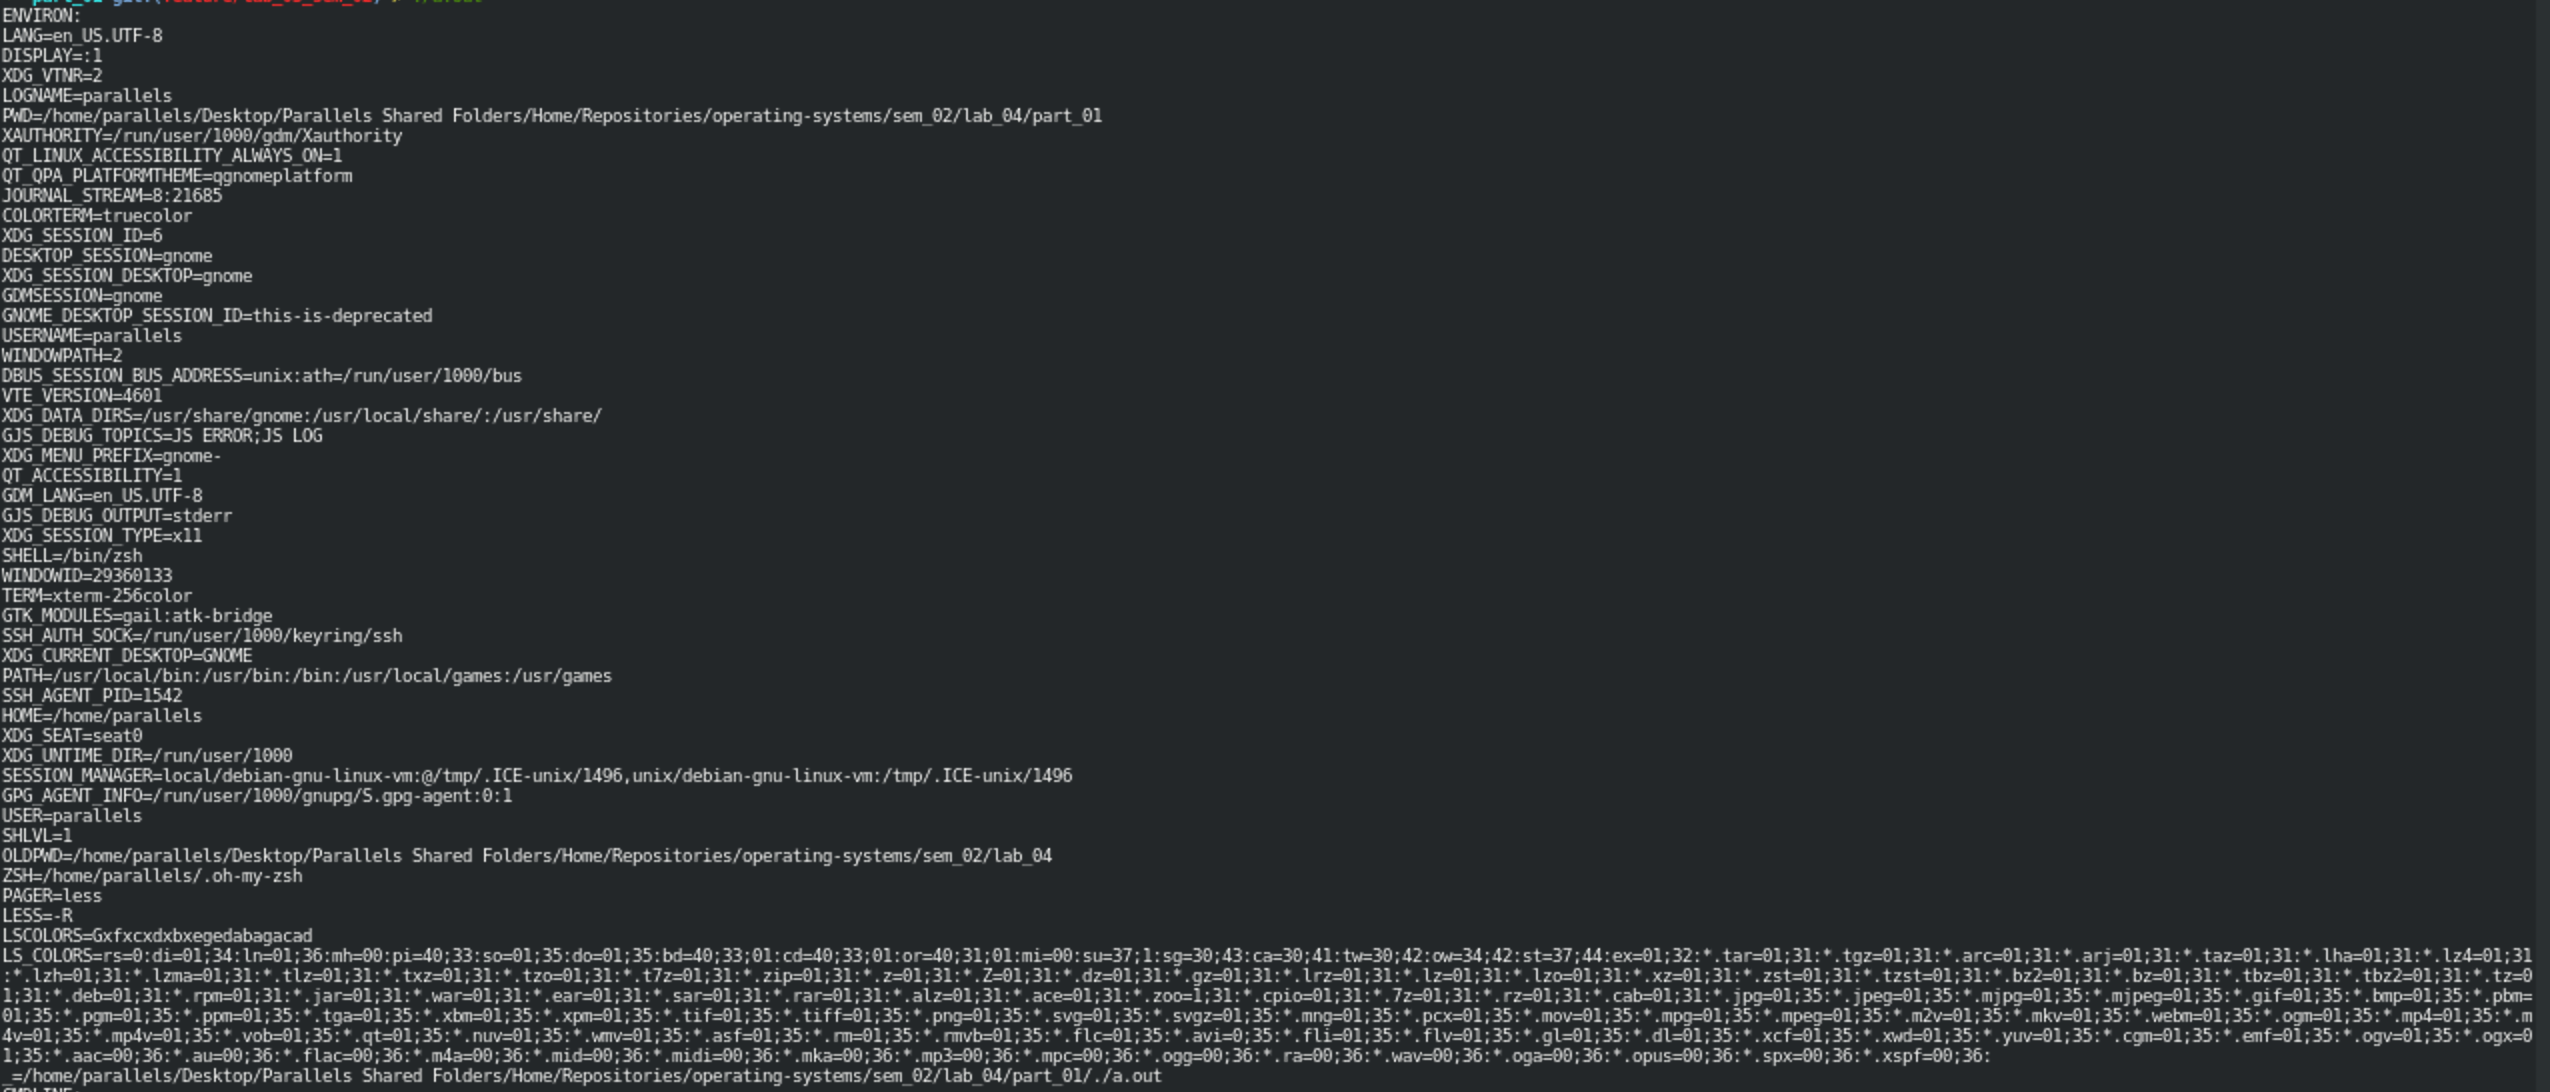
\includegraphics[scale=0.40]{img/part_01/env.png}
    \caption{Вывод информации об окружении процесса}
\end{figure}

\begin{figure}[H]
    \centering
    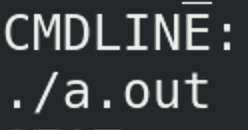
\includegraphics{img/part_01/cmdline.png}
    \caption{Вывод директории процесса (файл {\ttfamily cmdline})}
\end{figure}

\begin{figure}[H]
    \centering
    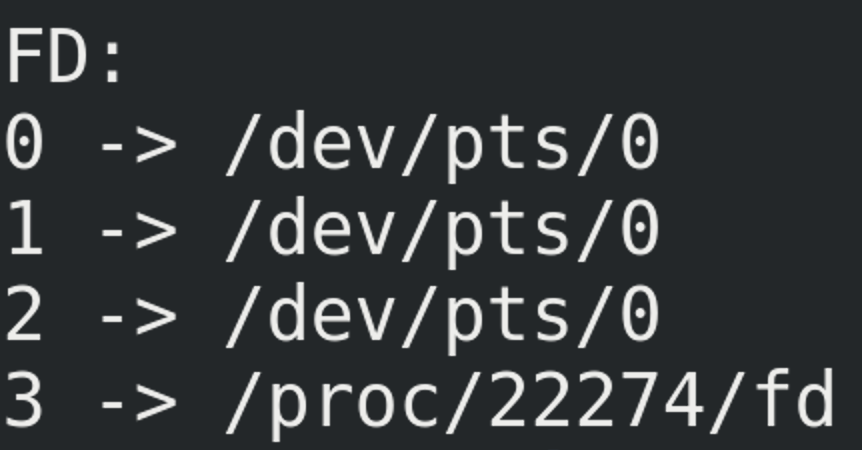
\includegraphics{img/part_01/fd.png}
    \caption{Вывод содержания директории {\ttfamily fd}}
\end{figure}

\begin{figure}[H]
    \centering
    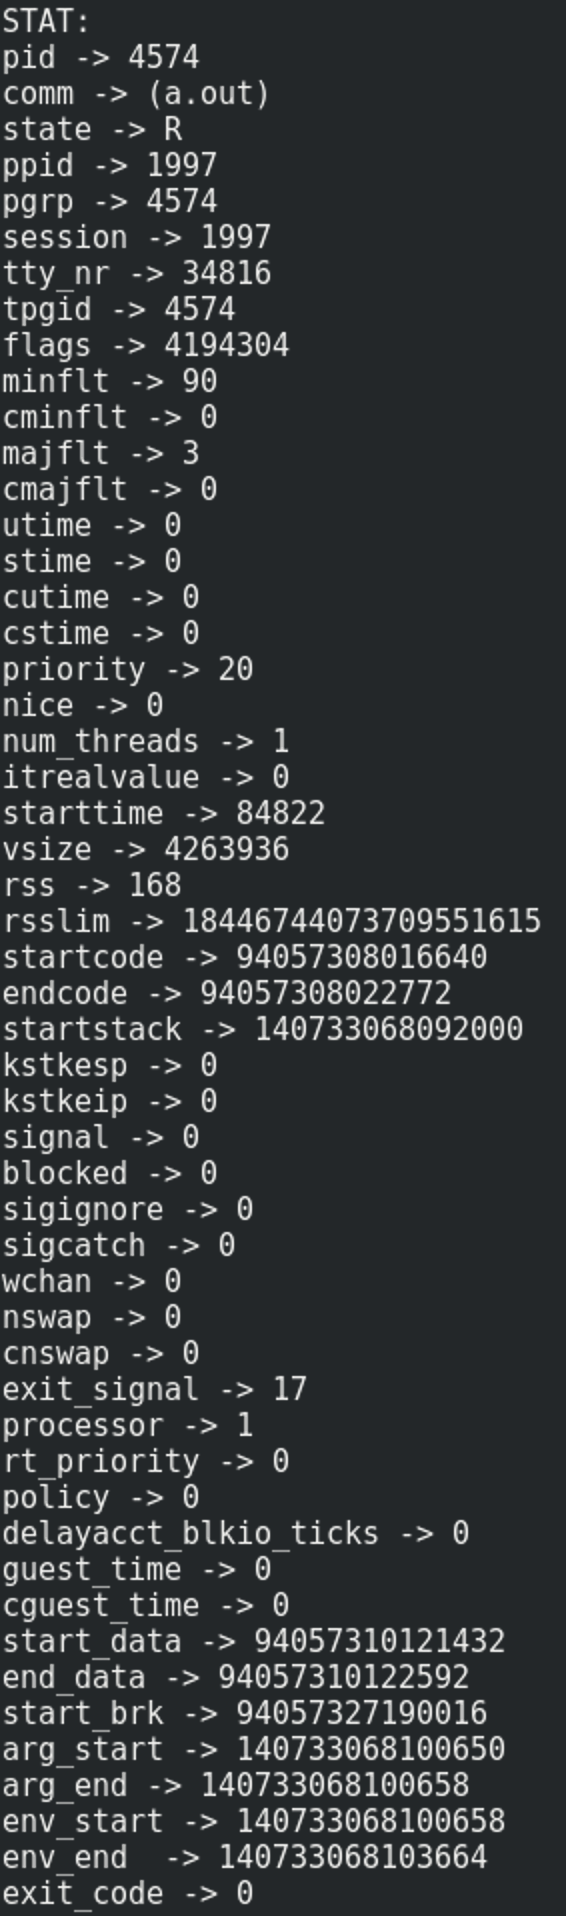
\includegraphics{img/part_01/stat.png}
    \caption{Вывод состояния процесса (файл {\ttfamily stat})}
\end{figure}
